\capitulo{REFERENCIAL TEÓRICO}

\secao{Problemas de Otimização}

Otimização é o processo de encontrar a melhor solução, também chamada de solução ótima para um determinado problema \cite{timoteo2005desenvolvimento}.\par

De acordo com \cite{steiglitz1982combinatorial} a constituição de um problema de otimização se deve aos termos vizinhança, ótimo local e ótimo global. O termo vizinhança se trata de um subconjunto do conjunto do problema, ótimo local pode ser tratado como o melhor resultado em uma vizinhança, e ótimo global é a melhor solução encontrada no conjunto de acordo com a função objetivo.\par

De acordo com a figura 1 pode se observar a relação entre ótimo local e ótimo global em um problema típico de minimização.\par

\begin{figure}[!htb]
\caption[Representação de um problema de minimização com ótimos locais]{Representação de um problema de minimização com ótimos locais}
\label{fig:figura2}
\centering
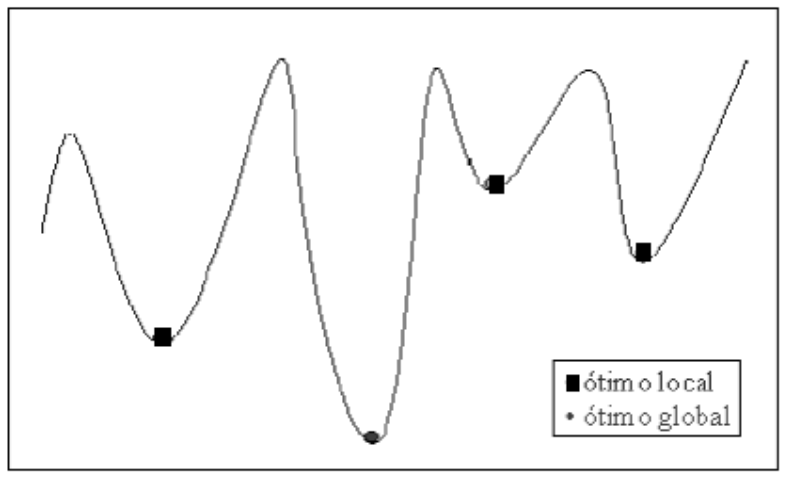
\includegraphics[scale=0.55]{imagens/problemaOtimizacao.png}
\\ \textbf{\footnotesize Fonte: \cite{timoteo2005desenvolvimento}}
\end{figure}

Segundo \cite{steiglitz1982combinatorial}, os problemas de otimização são divididos em duas categorias, problemas com variáveis contínuas e problemas com variáveis discretas. Problemas com variáveis discretas também podem ser conhecidos como Problemas de Otimização Combinatória (POC).\par

Conforme cita \cite{raupp2003introduccao}, o problema de otimização combinatória pode ser denominado como a ação de maximizar ou minimizar uma função objetiva de diversas variáveis sujeita a um conjunto de restrições, dentro de um contexto.\par

De acordo com \cite{opac-b1092847} problemas do tipo POC tratam do estudo matemático para encontrar agrupamentos, arranjos ou a seleção ótima de objetos discretos, logo, não permitindo, a utilização de métodos clássicos de otimização contínua para sua resolução.\par


Segundo \cite{golbarg2000otimizaccao} a ocorrência de problemas de otimização combinatória podem acontecer em diversas áreas, projetos de sistemas de distribuição de energia elétrica, posicionamento de satélites, roteamento ou escalonamento de veículos, sequenciamento de genes e DNA, classificação de plantas e animais.\par

De acordo com \cite{deleonardo} em problemas de otimização combinatória, cujo universo de dados é grande e existe um grande número de combinações, o que torna inviável a análise de todas soluções possíveis em um tempo adequado, utilizamos as heurísticas, também conhecidas como algoritmos heurísticos, que são métodos que compõem uma gama de soluções para problemas de otimização combinatória.

\secao{Heurística}

O termo heurística é derivado do grego \textit{heuriskein}, o que significa descobrir ou achar. De acordo com \cite{timoteo2005desenvolvimento} o significado da palavra em pesquisa operacional vai um pouco além da raiz etimológica. Segundo \cite{steiglitz1982combinatorial}, heurísticas são consideradas métodos de aproximação ou métodos de busca de solução, deve se levar em consideração que não exista uma garantia formal de seu desempenho e uma garantia de que estas heurísticas que iram encontrar uma solução. As heurísticas, apesar de não garantirem encontrar a solução ótima para um problema, procuram por soluções consideradas de boa qualidade em um tempo computacional razoável.\par

Segundo \cite{evans1992optimization} heurísticas são necessárias para implementação de problemas NP Difícil, caso deseje-se resolver tais problemas em um tempo  razoável.\par

Ressalta-se que dentre as heurísticas, as chamadas meta-heurísticas, merecem especial atenção pois adotam técnicas para amenizar, a dificuldade que os métodos heurísticos têm de escapar dos ótimos locais. As meta-heurísticas podem partir em busca de regiões mais promissoras no espaço de soluções, alem disto, as meta-heurísticas possuem grande abrangência, podendo ser aplicada à maioria dos problemas de otimização combinatória.\cite{nascimento2005aplicaccao}\par

Segundo \cite{adrianocesar} uma heurística é a instanciação de uma meta-heurística, ou seja, a aplicação da mesma em um problema específico de otimização.\par

Como exemplos de meta-heurísticas temos Busca Tabu (\textit{Tabu Search}), Otimização por Colônias de Formigas (\textit{Ant Colony Optimization}), Recozimento Simulado (\textit{Simulated Annealing}) e Algoritmo Genético (\textit{Genetic Algorithm}).\par

\subsecao{Busca Tabu}

%O que é

Busca tabu (BT) é uma meta-heurística adaptativa, que utiliza uma estrutura de memória através de uma lista, contendo um histórico de evolução para evitar que o processo de busca forme ciclos, ou seja, o retorno a um ótimo local previamente visitado \cite{souza2000} , \cite{armentanointroduccao} e \cite{subramanian2006aplicaccao}.\par


%Histótiria

Segundo \cite{subramanian2006aplicaccao} BT foi desenvolvida por \cite{glover1986future} com o objetivo de encontrar soluções para problemas de programação linear. Ao formalizar a técnica, o autor publicou uma serie de trabalhos envolvendo diversas aplicações da meta-heurística. \par

%Funcionamento

Basicamente o funcionamento do BT a feito partir da definição de uma população inicial ${S_0}$, o algoritmo explora cada iteração, de um subconjunto V da vizinhança N(S) da solução corrente S. O membro S’ de V com melhor valor nessa região segundo a função f(.) torna-se a nova solução corrente mesmo que S’ seja pior que S isto é, que f(S’) $>$ f(S) para um problema de minimização\cite{souza2000}. A figura 2 representa o pseudocódigo do algorítimo da Busca Tabu.

%Caracteristicas

Segundo \cite{armentanointroduccao}  o algorítimo tem um intensivo uso de memória o que é uma característica essencial deste método. Para o autor o uso da memória pode ajudar a intensificar a busca em regiões com grande chances de se encontrar o resultado, ou até mesmo, diversificar a busca através de regiões inexploradas.
\begin{figure}[!htb]
\caption[Representação do pseudocódigo do algorítimo da Busca Tabu]{Representação do pseudocódigo do algorítimo da Busca Tabu}
\label{fig:figura2}
\centering
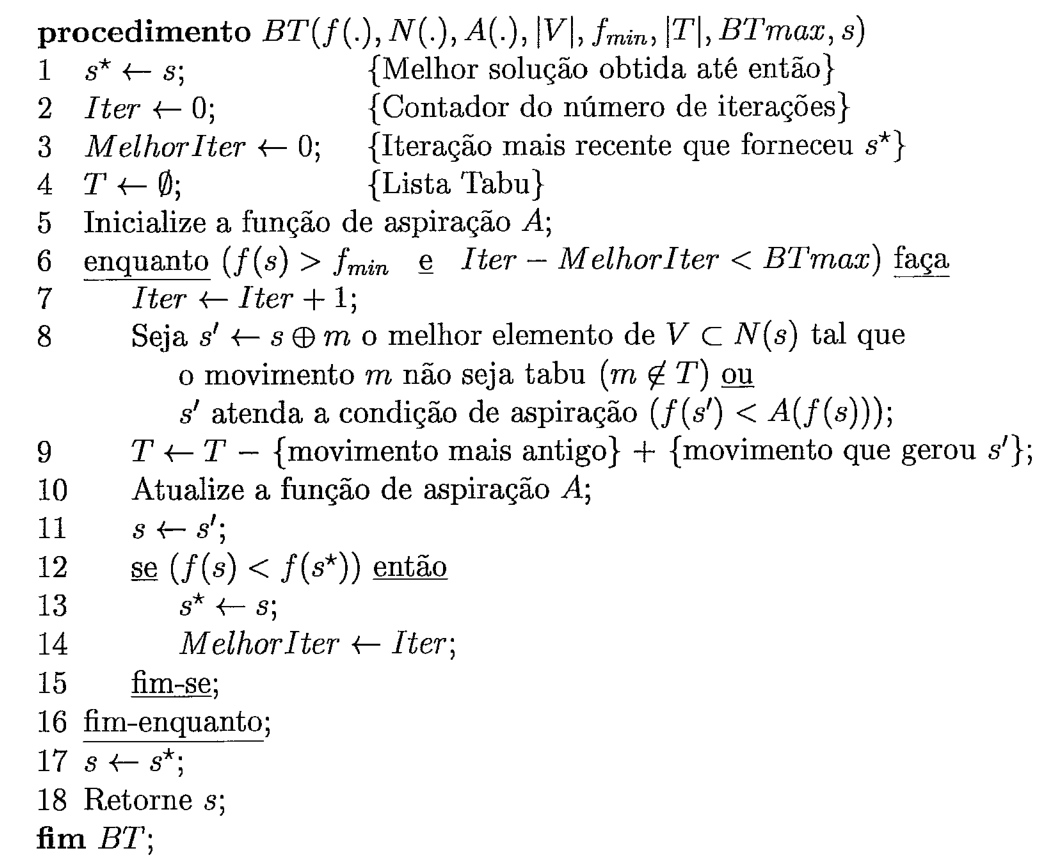
\includegraphics[scale=0.50]{imagens/representacaoBuscaTabu.png}
\\ \textbf{\footnotesize Fonte: \cite{souza2000}}
\end{figure}

De acordo com \cite{armentanointroduccao}  devemos adotar alguns procedimentos para que o processo de busca tenha um melhor resultado, listas tabu dinâmicas, passagens por regiões planas, intensificação, diversificação,\textit{path relinking}. Listas tabu dinâmicas tem como objetivo evitar que o algorítimo entre em processo de ciclo.Passagens por regiões planas pode levar o algorítimo a pensar que não existem melhoras significativas na qualidade das soluções e atingir o critério de parada, para evitar esta situação é necessário aumentar o tamanho da lista tabu enquanto o algorítimo estiver passando pela região plana e voltar a reduzir quando houver mudança no valor da função objetiva.Intensificação são técnicas utilizadas para concentrar os esforços da pesquisa em regiões consideradas promissoras. Diversificação é uma técnica que utiliza memória de longo prazo para redirecionar a pesquisa para regiões que ainda não foram suficientemente exploradas. PathRelinking trada ta intensificação de incorporar atributos de soluções de boa qualidade (chamadas de soluções elite), em seguida explora caminhos que contenham uma ou mais soluções de elite.

Ainda segundo \cite{armentanointroduccao} uma característica importante do método é que a solução final tem pouca ou nenhuma dependência da escolha feita para a solução inicial, isso graças aos mecanismos implementados pelo método, que fogem de ótimos locais.

\subsecao{Recozimento Simulado}

%O que é
%Histótiria
%Caracteristicas
Técnica de busca local probabilística, proposta originalmente por \cite{kirkpatrick1983optimization}, que se fundamenta em uma analogia com a termodinâmica, ao simular o 
resfriamento de um conjunto de átomos aquecidos. Isto é, conforme \cite{noronha2003abordagem} em 
analogia a física da matéria: levando um cristal a sua temperatura de fusão, as moléculas 
estão desordenadas e se agitam livremente. Ao resfriar-se a amostra de maneira 
infinitamente lenta, as moléculas vão adquirir a estrutura cristalina estável que tem um 
nível de energia mais baixo possível. 
Conforme \cite{aarts1988simulated} a analogia com a otimização (combinatória ou não) 
é bastante direta. Os estados da matéria são as soluções realizáveis, a quantidade objetiva 
substitui a energia, os estados metaestáveis da matéria sendo ótimos locais e a estrutura 
cristalina corresponde ao ótimo global. 
Segundo \cite{reeves1993modern}, a temperatura Tassume, inicialmente, um valor 
elevado T0e o procedimento pára quando a temperatura chega a um valor próximo de zero 
e nenhuma solução que piore o valor da função objetivo é mais aceita, isto é, quando o 
sistema está estável.\par
Mais informações em \cite{reeves1993modern} e \cite{kirkpatrick1983optimization}. 

\subsecao{Algoritmos genéticos}

Conforme cita \cite{oliveira2005algoritmo}, os algoritmos genéticos foram introduzidos 
por \cite{holland1975adaptation}, com intuito de aplicar a teoria da evolução das espécies 
elaborada por \cite{darwin1968origin} utilizando os conceitos da evolução biológica como 
genes, cromossomos, cruzamento, mutação e seleção na computação procurando explicar rigorosamente processos de adaptação em sistemas naturais e desenvolver sistemas artificiais (simulados em computador) que mantenham os mecanismos originais, encontrados em sistemas naturais.\par

Segundo \cite{oliveira2005algoritmo}, o processo de evolução executado por um algoritmo genético corresponde a um procedimento de busca no espaço de soluções potenciais para o problema e, como enfatiza \cite{michalewicz1996evolutionary}, esta busca requer um equilíbrio entre dois objetivos aparentemente conflitantes: a procura das melhores soluções na região que se apresenta promissora ou fase de intensificação e a procura de outra região ou exploração do espaço de busca, também conhecida como diversificação.\par
Ainda segundo \cite{oliveira2005algoritmo}, os algoritmos genéticos têm se mostrado ferramentas poderosas para resolver problemas onde o espaço de busca é muito grande e os métodos convencionais se mostraram ineficientes.\par

Mitchel \cite{mitchell1998introduction} cita que a terminologia biológica é muito importante para a compreensão do funcionamento dos algoritmos genéticos. Eis os principais termos: \par
•  Cromossomo: estrutura que representa uma determinada característica da solução ou a própria solução; \par
•  Gene: característica particular de um cromossomo. O cromossomo é composto por um ou mais genes. \par
•  Alelo: valor de determinado gene;\par
•  Locus: determinada posição do gene no cromossomo;\par
•  Genótipo: estrutura que codifica uma solução. Um genótipo pode ser formado por um ou mais cromossomos; \par
•  Fenótipo: decodificação ou o significado da estrutura; \par
•  Fitness: significa aptidão. O quanto o indivíduo é apto para determinado ambiente; \par
As principais características que diferenciam os algoritmos genéticos de métodos tradicionais são \cite{goldberg1989genetic}: \par
•  Parâmetros: os algoritmos genéticos trabalham com a codificação dos parâmetros e não com os parâmetros propriamente; \par
•  Número de soluções: os algoritmos genéticos trabalham com uma população de indivíduos (representando um conjunto de soluções) e não com uma única solução; \par

•  Avaliação das soluções: os algoritmos genéticos utilizam informações de custo ou recompensa penalizando ou premiando determinadas características das soluções; \par

•  Regras: os algoritmos genéticos utilizam regras probabilísticas e não determinísticas; \par

O algoritmo genético é uma forma da estratégia gerar-e-testar realizando os testes baseados nos parâmetros da evolução biológica. Uma desvantagem notável é a variação dos operadores genéticos do algoritmo em cada problema. Dessa forma, para resolução de determinado problema, torna-se necessário um estudo particular a respeito do mesmo. \par

O algoritmo genético atua sobre uma população fazendo com que esta evolua de acordo com uma função de avaliação. O funcionamento é iterativo iniciando com a geração de uma população inicial que pode ser aleatória ou não, seguida do processo de avaliação, seleção, cruzamento e mutação, que ocorre a cada iteração até que seja atingido algum critério de parada. Os passos gerais de um algoritmo genético são ilustrados na figura 
Figura XXXX. Cada passo pode ser realizado de várias maneiras e pode variar de problema para problema \cite{timoteo2005desenvolvimento}.\par 

Figura Etapas de um Algoritmo Genético Básico 

\secao{TimeTabling}

Segundo \cite{kripkasimulated} os problemas de programação de horários (PPH), também conhecidos como \textit{TimeTabling}, são os problemas que mais se destacam nas organizações acadêmicas. De acrodo com \cite{schaerf1999survey} estes problemas são divididos em três categorias \textit{school timetabling}, \textit{course timetabling} e \textit{examination timetabling}.\par

\textit{School TimeTabling}: Se trata basicamente da geração de horários semanais, em escolas de segundo grau, onde deve-se evitar os choques entre os horários das disciplinas e que cada professor receba apenas uma turma para cada horário. Neste caso o aluno recebe um número fixo de disciplinas a serem cursadas.\par

\textit{Course TimeTabling}: Diz respeito à alocação de aulas de uma universidade típica. Neste problema os alunos podem escolher as matérias em que vão se matricular, portando o problema tem como objetivo minimizar os possíveis choques entre as disciplinas, professores e horários disponibilizados pela instituição de ensino.\par

\textit{Examination TimeTabling}: Aborda o problema de programação de horários dos exames da instituição, de maneira que, disciplinas que tenham alunos em comum, distanciem o máximo possível as datas dos exames.\par

Segundo \cite{pinheiro2001ambiente} o problema de programação de horários vem sendo abordado desde a década de 60, sendo que os primeiros trabalhos a se destacarem foram realizados na década de 80.\par

O Problema de Alocação de Salas (PAS) também conhecido como \textit{Classroom Assignment} é tratado como parte do problema de programação de cursos universitários \textit{course timetabling}. Segundo \cite{marinho2005heuristicas} varias instituições universitárias se deparam com o PAS durante o início de cada semestre letivo, este problema é considerado NP-Difícil por \cite{even1975complexity} e \cite{carter1992classroom}, com isto, a determinação da solução ótima do problema, em um período de tempo aceitável se torna uma tarefa difícil.\par
Segundo \cite{kripkasimulated} o problema deve considerar que as disciplinas dos cursos universitários já tenham seus horários de início e de término definidos. O problema se resume então na alocação das disciplinas às salas desta universidade respeitando os horários destas disciplinas e as demais restrições exigidas.

Segundo \cite{souza2000} boa parte das universidades ainda resolvem este problema de forma manual, o que torna o processo árduo e demorado, podendo levar vários dias para ser concluído.\par

Uma vez que é de extrema dificuldade encontrar a solução ótima do PAS em tempo razoável, este problema é normalmente tratado através de técnicas heurísticas, que apesar de não garantirem encontrar a solução ótima do problema, são capazes de retornar uma solução de qualidade em um tempo adequado. As meta-heurísticas surgiram como uma alternativa para amenizar a dificuldade que os métodos heurísticos tem de escapar dos chamados ótimos locais.\cite{nascimento2005aplicaccao}.\par

Segundo \cite{even1975complexity} o PAS pertence a classe de Problemas de Otimização Combinatória (POC).\par


\secao{Trabalhos Relacionados}
trabalho do marinho que usa tabu.
trabalho da silvia que usa Recozimento Simulado (Simulated Annealing).
trabalho da leonardo que usa Algoritmos Genéticos (AG).
achar algum trabalho que utiliza o algoritimo das formigas.
falar porque o trabalho do cara se assemelha ao meu trabalho.